\documentclass[11pt]{article}

\usepackage{amsmath}
\usepackage{amssymb}
\usepackage{array}
\usepackage{geometry}
\usepackage{enumitem}
\usepackage{float}
\usepackage{cancel}
\usepackage{graphicx}
\usepackage[labelformat=empty]{caption}
\usepackage{booktabs}

\geometry{
	a4paper,
 	left=20mm,
 	top=20mm,
 	bottom=20mm,
}

\setlength{\parindent}{0pt}

\begin{document}

\section{Wahrscheinlichkeiten}

\begin{table}[H]
\centering
\begin{tabular}{|p{2cm}|p{6cm}|p{6cm}|}
\hline
                   & \textbf{with repetition} & \textbf{without repetition} \\\hline
\textbf{ordered}   & $n^k$                         							 	  & $\frac{n!}{(n-k)!}$    \\\cline{2-3}
				   & A passcode of length $n$ with $k$ different digits           & How many ways can $k$ places be awarded to $n$ people                       \\\hline
\textbf{unordered} & $\bigl(\begin{smallmatrix}n+k-1\\k \end{smallmatrix} \bigr)$ & $\bigl(\begin{smallmatrix}n\\k \end{smallmatrix} \bigr) = \frac{n!}{k!(n-k)!}$ \\\cline{2-3}
				   & Distribute $k$ bananas (identical) to $n$ monkeys (identical)   & Select $k$ from $n$ objects                             \\\hline
\end{tabular}
\end{table}

\begin{description}[labelindent=16pt,style=multiline,leftmargin=9cm, noitemsep]
	\item[Ereignisraum $\Omega$:] Die Menge aller m{\"o}glichen Ergebnisse
	\item[Elementarereignis $\omega \in \Omega$:] Elemente vom Ereignisraum
	\item[Potenzmenge $\mathcal{P}(\Omega)$ oder $2^\Omega$:] Menge aller Teilmengen von $\Omega$
	\item[prinzipielles Ereigniss $A \subseteq \Omega$:] Kollektion von Elementarereignissen
	\item[Klasse der beobachtbaren Ereignisse $\mathcal{F}$:] Teilmenge der Potzenmenge $\mathcal{P}(\Omega)$ (alle m{\"o}glichen Ereignisse)
	\item[Wahrscheinlichkeitsmass $P: \mathcal{F} \mapsto \lbrack 0,1 \rbrack $:] Weist einem Ereignis eine Wahrscheinlichkeit zu
\end{description}

Es gelten:
\begin{equation*}
\begin{split}
	P[A^c] & = 1 - P[A] \\
	P[A \cup B] & = P[A] + P[B] - P[A \cap B] \quad\text{(Additionsregel)} \\
	P[A \cap B] & = P[B|A] \cdot P[A] \quad\text{(Multiplikationsregel)} \\
	P[A \backslash B] & = P[A] - P[A \cap B] \\
	P[A \cap B \cap C] + P[A \cap B \cap C^c] & = P[A \cap B]
\end{split}
\end{equation*}

\subsection{Diskrete Wahrscheinlichkeitsr{\"a}ume}

Ist $\Omega = {\omega_1, \omega_2,...,\omega_N}$ endlich mit $|\Omega| = N$ und $\mathcal{F} = 2^\Omega$ und sind die Elementarereignisse alle gleich wahrscheinlich, so ist $\Omega$ ein \textbf{Laplace-Raum} und $P$ die \textbf{diskrete Gleichverteilung} auf $\Omega$.

\begin{equation*}
	P[A] = \frac{\text{Anzahl der Elementarereignisse in A}}{\text{Anzahl der Elementarereignisse in $\Omega$}} = \frac{|A|}{|\Omega|}
\end{equation*}

\subsection{Bedingte Wahrscheinlichkeiten}

Die bedingte Wahrscheinlichkeit von $B$ unter der Bedingung, dass $A$ eintritt ($A$ gegeben) ist definiert durch:
\begin{equation*}
\begin{split}
	P[B|A] & := \frac{P[B \cap A]}{P[A]} \\
	P[B^c|A] & = 1-P[B|A] \\
\end{split}
\end{equation*}

\emph{Veranschaulichung:} $A$ ist eingetreten. Da $A$ und $B$ von einander abh{\"a}ngen, l{\"a}sst sich somit auch die Wahrscheinlichkeit berechnen, dass $B$ eingetreten ist.

\paragraph{Satz der totalen Wahrscheinlichkeit:} Sei $A_1,...,A_n$ eine Zerlegung von $\Omega$ in paarweise disjunkte Ereignisse, dann gilt f{\"u}r ein beliebiges Ereignis $B$:
\begin{equation*}
	P[B] = \sum_{i=1}^n P[B|A_i] P[A_i]
\end{equation*}
\begin{center}
	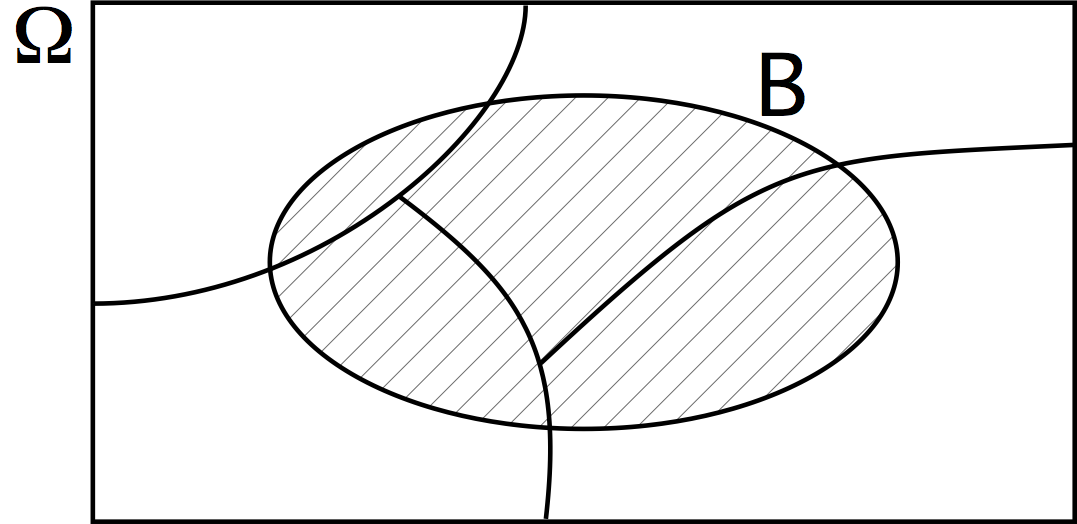
\includegraphics[width=200pt]{images/totale_wahrscheinlichkeit}
\end{center}

\paragraph{Formel von Bayes:} Ist $A_1,...,A_n$ eine Zerlegung von $\Omega$ mit $P[A_i] > 0$ und $B$ ein Ereignis mit $P[B] > 0$ so gilt f{\"u}r jedes $k$:
\begin{equation*}
	P[A_k|B] = \frac{P[B|A_k]P[A_k]}{\sum_{i=1}^n P[B|A_i]P[A_i]}
\end{equation*}

\subsection{Unabh{\"a}ngigkeit}

Zwei Ereignisse $A, B$ sind unabh{\"a}ngig (stochastisch), falls gilt:
\begin{equation*}
\begin{split}
	P[A \cap B] & = P[A]P[B] \quad\text{(Produktregel)}\\
	P[B|A] & = P[B] \\
	P[A|B] & = P[A] \\
\end{split}
\end{equation*}

\emph{Veranschaulichung:} Die Tatsache, dass eines der Ereignisse eingetreten ist, hat keinen Einfluss auf die Wahrscheinlichkeit des anderen. Unabh{\"a}ngigkeit und disjunkte Mengen sind jedoch \emph{nicht} das selbe.

\section{Diskrete Zufallsvariablen und Verteilungen}

\begin{description}[labelindent=16pt,style=multiline,leftmargin=8cm, noitemsep]
	\item[Zufallsvariable $X: \Omega \mapsto \mathbb{R}$:] Eine eindeutige Zuordnung, die jedem Elementarereignisses im Ereignisraum eine Zahl zuordnet.
	\item[Verteilungsfunktion $F_X: \mathbb{R} \mapsto \lbrack 0,1 \rbrack$:] $F_X(t) := P[X \leq t] := P[\{\omega | X(\omega) \leq t\}]$ \\ Der Wert an der Stelle $x$  entspricht der Wahrscheinlichkeit, dass die zugeh{\"o}rige Zufallsvarible $X$ einen Wert kleiner oder gleich $x$ annimmt.
	\item[Gewichtsfunktion $p_X:\mathcal{W}(X) \mapsto \lbrack 0,1 \rbrack$:] $p_X(x_k) := P[X = x_k] = P[\{\omega | X(\omega) = x_k\}]$ \\ Die Summe aller Gewicht aller Ereignisse muss zusammen 1 ergeben.
	\item[Indikatorfunktion $I_A$:] $I_A(\omega) = 1$, falls $\omega \in A$, $0$ sonst. Eine diskrete Zufallsvariable, falls $\Omega$ endlich und abz{\"a}hlbar ist.
\end{description}

\subsection{Erwartungswert}

Sei $X$ eine diskrete Zufallsvariable mit Gewichtsfuntkion $p_X(x)$, dann ist der Erwartungswert $E[X]$ wie folgt definiert:
\begin{equation*}
	E[X] := \sum_{x_k \in \mathcal{W}(X)} x_kp_X(x_k)
\end{equation*}

Ist diese Reihe nicht \emph{absolut konvergent}, so existiert der Erwartungswert nicht.

Sei weiter $Y = g(X)$ eine Zufallsvariable gem{\"a}ss $g: \mathbb{R}\mapsto\mathbb{R}$ abh{\"a}ngig von $X$, so gilt:
\begin{equation*}
	E[Y] = E[g(X)] = \sum_{x_k \in \mathcal{W}(X)} g(x_k)p_X(x_k)
\end{equation*}

F{\"u}r zwei Zufallsvariablen $X$ und $Y$, die jeweils einen Erwartungswert definiert haben, gilt:
\begin{description}[labelindent=16pt,style=multiline,leftmargin=4cm, noitemsep]
	\item[Monotonie:] Ist $X \leq Y$ (bzw. $\forall\omega: X(\omega) \leq Y(\omega)$), so gilt auch $E[X] \leq E[Y]$
	\item[Linearit{\"a}t:] F{\"u}r beliebige $a,b \in \mathbb{R}$ gilt $E[aX + b] = aE[X]+b$
	\item[Werte in $\mathbb{N}_0$:] Falls $X$ nur Werte in $\mathbb{N}_0$ annimmt, so gilt \\ $E[X] = \sum^\infty_{j=1}P[X \geq j] = \sum^\infty_{l=0}P[X > l]$
\end{description}

\subsection{Varianz}

Sei $X$ eine diskrete Zufallsvariable und ist $E[X] < \infty$, so ist die \textbf{Varianz} definiert als:
\begin{equation*}
	\text{Var}[X] := E[(X-E[X])^2] = \sum_{x_k \in \mathcal{W}(X)}(x_k - E[X])^2 p_X(x_k)
\end{equation*}

Dementsprechend ist die \textbf{Standardabweichung} von $X$ gleich
\begin{equation*}
	\text{sd}(X) = \sigma(X) := \sqrt{\text{Var}[X]}
\end{equation*}

Die Varianz wie auch die Standardabweichung beschreiben die \textbf{Streuung} der Verteilung von $X$. F{\"u}r beliebiges $X$ und $Y = aX +b$ gilt:

\begin{equation*}
\begin{split}
	\text{Var}[X] & = E[X^2] - E[X]^2 \\
	\text{Var}[Y] & = \text{Var}[aX +b] = a^2\text{Var}[X]
\end{split}	
\end{equation*}

\subsection{Gemeinsame Verteilungen}

\begin{equation*}
\begin{split}
	\text{Gemeinsame Gewichtsfunktion } p: \mathbb{R}^n \mapsto [0,1] \qquad & p(x_1,...,x_n) := P[X_1 = x_1,..., X_n = x_n] \\
	\text{Gemeinsame Verteilungsfunktion } F: \mathbb{R}^n \mapsto [0,1] \qquad & F(x_1,...,x_n) = P[X_1 \leq x_1,..., X_n \leq x_n] \\
	& = \sum_{y_1 \leq x_1,...,y_n \leq x_n} p(y_1,...,y_n)
\end{split}
\end{equation*}

\emph{Veranschaulichung:} F{\"u}r die Zufallsvariablen $X$ und $Y$ beschreibt die gemeinsame Verteilungsfunktion die Wahrscheinlichkeit, dass der Vektor $(X,Y)$ in ein unendliches Rechteck der Form $(-\infty, X] \times (-\infty,y]$ f{\"a}llt.

\subsubsection{Randverteilungen}

Haben $X$ und $Y$ die gemeinsame Verteilungsfunktion $F$, so ist die Verteilungsfunktion der Randverteilung von $X$ gegeben durch:
\begin{equation*}
	F_X(x) := P[X \leq x] = P[X \leq x, Y < \infty] = \lim_{y \rightarrow \infty} F(x,y)
\end{equation*}

Analog dazu ist die Gewichtsfunktion der Randverteilung von $X$ gleich:
\begin{equation*}
	p_X(x) = P[X = x] = \sum_{y_i \in \mathcal{W}(Y)} P[X=x, Y=y_i] = \sum_{y_i \in \mathcal{W}(Y)} p(x, y_i) \text{ f{\"u}r } x \in \mathcal{W}(X)
\end{equation*}

\subsubsection{Unabh{\"a}ngigkeit}

Die Zufallsvariablen $X_1,...,X_n$ heissen \textbf{unabh{\"a}ngig}, falls
\begin{equation*}
\begin{split}
		\text{entweder} \quad & F(x_1,...,x_n) = F_{X_1}(x_1) \cdot\cdot\cdot F_{X_n}(x_n)  \\
		\text{oder} \quad & p(x_1,...,x_n) = p_{X_1}(x_1) \cdot\cdot\cdot p_{X_n}(x_n)
\end{split}
\end{equation*}

\begin{equation*}
	\text{unabh{\"a}ngig} \Rightarrow \text{paarweise unabh{\"a}ngig} \Rightarrow \text{unkorreliert}
\end{equation*}

\subsection{Funktionen von mehreren Zufallsvariablen}

Seien $X_1,...,X_n$ diskrete Zufallsvariablen mit endlichen Erwartungswerten $E[X_1],...,E[X_n]$...

\subsubsection{Summen von Erwartungswerte}

Sei weiter $Y = a + \sum_{l=1}^n b_lX_l$ mit Konstanten $a,_1,...,b_n$, dann gilt:
\begin{equation*}
	E[Y] = a + \sum_{l=1}^n b_lE[X_l]
\end{equation*}

Es folgt, dass Erwartungswerte sich \textbf{immer linear verhalten}. Der Erwartungswert einer Summe von Zufallsvariablen ist also immer die Summe der Erwartungswerte.
	
\subsubsection{Summen von Varianzen}

Die \textbf{Kovarianz} von $X$ und $Y$ ist wie folgt definiert:
\begin{equation*}
	\text{Cov}(X,Y) = E[XY] - E[X]E[Y] = E[(X - E[X])(Y-E[Y])]
\end{equation*}

Es gelten:
\begin{equation*}
\begin{split}
	& \text{Cov}(X, X) = \text{Var}(X) \\
	& \text{Cov}(X, Y) = 0 \Rightarrow \text{$X$ und $Y$ sind unkorreliert}
\end{split}
\end{equation*}

Daraus folgt die \textbf{allgemeine Summenformel f{\"u}r Varianzen}:

\begin{equation*}
\begin{split}
	\text{korreliert:} \quad & \text{Var}\Bigg[\sum_{i=1}^n X_i \Bigg] = \sum_{i=1}^n\text{Var}[X_i] + 2\sum_{i<j}\text{Cov}(X_i, X_j) \\
	\text{unkorreliert:} \quad & \text{Var}\Bigg[\sum_{i=1}^n X_i \Bigg] = \sum_{i=1}^n\text{Var}[X_i]
\end{split}
\end{equation*}

\subsubsection{Produkte von Zufallsvariablen und Varianzen}

Falls $X_1,...X_n$ unabh{\"a}ngig sind und der Erwartungswert links {\"u}berhaupt existiert, gilt

\begin{equation*}
	E\Bigg[\prod_{i=1}^n X_i\Bigg] = \prod_{i=1}^n E[X_i]
\end{equation*}

In diesem Fall sind dann $X_1,...,X_n$ paarweise unkorreliert.

\subsection{Bedingte Verteilungen}

Seien $X$ und $Y$ diskrete Zufallsvariablen mit gemeinsamer Gewichtsfunktion $p(x, y)$. Die bedingte Gewichtsfunktion von $X$, gegeben dass $Y = y$, ist definiert durch
\begin{equation*}
	p_{X|Y}(x|y) := P[X=x|Y=y] = \frac{P[X=x,Y=y]}{P[Y=y]} = \frac{p(x,y)}{p_Y(y)}
\end{equation*}

\section{Wichtige Diskrete Verteilungen}



\end{document}
